\textbf{\textit{Definición: }} Todos los estimadores CAN que se obtienen usando el $\Delta$-método a partir de otro estimador AE, son AE.

\begin{proofs}
    Sea $T_n(X)$ estimador CAN para $\theta$
    \[
        \sqrt{n}(T_n(X)-\theta) \overset{L}{\to}N(0,V^2_T(\theta))
    \]

    y $T_n(X)$ es AE entonces

    \[
        V^2_T(\theta) = \frac{1}{I_T(\theta)} \implies I_T(\theta)=\frac{1}{V^2_T(\theta)}
    \]

    Sea $g$ una función con derivada no nula, se tiene

    \[
        \sqrt{n}(g(T_n(X))-g(\theta)) \overset{L}{\to}N(0,V^2_T(\theta)(g'(\theta))^2)
    \]

    La varianza de $g(T_n(X))$ es

    \[
        Var(g(T_n(X)))=\frac{V^2_T(\theta)(g'(\theta))^2}{n}
    \]

    Y su cota CR es

    \[
        \frac{(g'(\theta))^2}{nI_{X_1}(\theta)}=\frac{(g'(\theta))^2}{\frac{n}{V^2_T(\theta)}}=\frac{V^2_T(\theta)(g'(\theta))^2}{n}\square
    \]
\end{proofs}


\section{Inferencia Basada en Verosimilitud}


\subsection{Caso Uniparamétrico}

Toda información acerca de $\theta$ que los datos nos proporcionan está en la función de verosimilitud.

\textbf{\textit{Definición: }} Sean $X_1, \dots, X_n$ v.a.i.i.d. Se define como función de verosimilitud a

\[
    L(\theta; X_1,\dots,X_n) =
    \begin{cases}
        P_\theta(X_1,\dots,X_n)=\prod_{i=1}^{n}P_\theta(X_i=x_i) & \text{Caso discreto} \\
        f(X_1,\dots,X_n; \theta)=\prod_{i=1}^{n}f(x_i; \theta)   & \text{Caso continuo}
    \end{cases}
\]

$L(\theta; X_1,\dots,X_n)$ es una función de $\theta$ proporcional a la probabilidad de observar que $(X_1,\dots,X_n)=(x_1,\dots,x_n)$ cuando $\theta$ es el verdadero valor del parámetro. Así, un valor del parámetro será más o menos verosimil cuanto mayor o menor sea esa verosimilitud.

\newpage

Consideremos las siguientes condiciones:

\begin{enumerate}
    \item El parámetro $\theta$ es identificable, es decir, que $\theta \neq \theta' \implies P_\theta \neq P_{\theta'}$
    \item Las distribuciones $P_\theta$ donde $\theta \in \Theta$ tienen el mismo soporte $\{x:f(x,\theta) > 0\}$ y no depende de $\theta$
\end{enumerate}

\textbf{\textit{Resultado: }} Sean $X_1,\dots,X_n$ v.a.i.i.d. con $f(X;\theta)$. Entonces si $\theta_0$ es el verdadero valor del parámetro

\[
    P_\theta(L(\theta_0;X_1,\dots,X_n)>L(\theta;X_1,\dots,X_n))\xrightarrow{n\to\infty}1
\]

\begin{proofs}
    Sea

    \[
        \left\{x:L(\theta_0;X_1,\dots,X_n)>L(\theta;X_1,\dots,X_n)\right\}=\left\{x:\prod_{i=1}^{n}\frac{f(x_i;\theta)}{f(x_i;\theta_0)}<1\right\}
    \]

    donde aplicando logaritmos

    \[
        \left\{x:\frac{1}{n}\sum_{i=1}^{n}\log{\frac{f(x_i;\theta)}{f(x_i;\theta_0)}}<0\right\}
    \]

    Tenemos que

    \[
        \frac{1}{n}\sum_{i=1}^{n}\log{\frac{f(x_i;\theta)}{f(x_i;\theta_0)}} \overset{P}{\to}E_{\theta_0}=\left(\log{\frac{f(x_i;\theta)}{f(x_i;\theta_0)}}\right)
    \]

    Aplicando la desigualdad de Jensen para funciones convexas: $f(E(X)) \leq E(f(X))$ donde $-\log$ es convexa

    \[
        E_{\theta_0}\left(-\log{\frac{f(x_i;\theta)}{f(x_i;\theta_0)}}\right) \geq -\log{E_{\theta_0}\left(\frac{f(x_i;\theta)}{f(x_i;\theta_0)}\right)} \implies
    \]

    \[
        \implies E_{\theta_0}\left(\log{\frac{f(x_i;\theta)}{f(x_i;\theta_0)}}\right) \leq \log{E_{\theta_0}\left(\frac{f(x_i;\theta)}{f(x_i;\theta_0)}\right)}
    \]

    Y como

    \[
        \log{E_{\theta_0}\left(\frac{f(x_i;\theta)}{f(x_i;\theta_0)}\right)}=\log\int\frac{f(x_i;\theta)}{f(x_i;\theta_0)}f(x_i;\theta_0)dx=\log\int f(x_i;\theta_0)dx=\log(1)=0
    \]

    probamos que $\frac{1}{n}\sum_{i=1}^{n}\log{\frac{f(x_i;\theta)}{f(x_i;\theta_0)}}$ converge a una cantidad negativa
\end{proofs}

\newpage

\subsubsection{Estimación por Máxima Verosimilitud}

El estadistico EMV es el valor en el que se alcanza el máximo de la verosimilitud o así mismo, puesto que la transformación logaritmica es monótona y creciente, de la log verosimilitud definida como $l(\theta;X_1,\dots,X_n)=\log L(\theta;X_1,\dots,X_n)$. \\

\textbf{\textit{Definición: }} $\hat{\theta}(x)$ será EMV de $\theta$ si

\[
    \hat{\theta}(x) = \underset{\theta \in \Theta}{argmax}(l(\theta;X_1,\dots,X_n))
\]

\begin{figure}[h!]
    \begin{minipage}{0.48\textwidth}
        \centering

        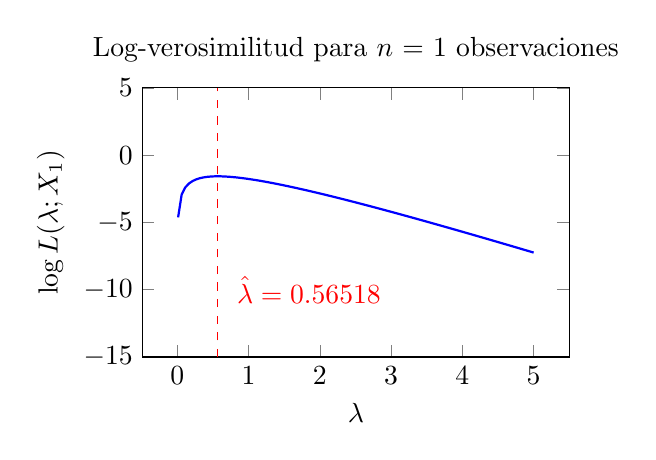
\begin{tikzpicture}
            \begin{axis}[
                    domain=0.01:5,
                    samples=100,
                    ymin=-15, ymax=5,
                    xlabel={$\lambda$},
                    ylabel={$\log L(\lambda; X_1)$},
                    title={Log-verosimilitud para $n$ = 1 observaciones},
                    width=7cm, height=5cm
                ]
                \addplot[thick,blue] {ln(x) - x*1.769362};
                \addplot[red, dashed] coordinates {(0.56518, -15) (0.56518, 5)};.
                \node at (axis cs: 0.7, -10) [anchor=west, red] {$\hat{\lambda} = 0.56518$};
            \end{axis}
        \end{tikzpicture}

    \end{minipage}
    \hfill
    \begin{minipage}{0.48\textwidth}
        \centering

        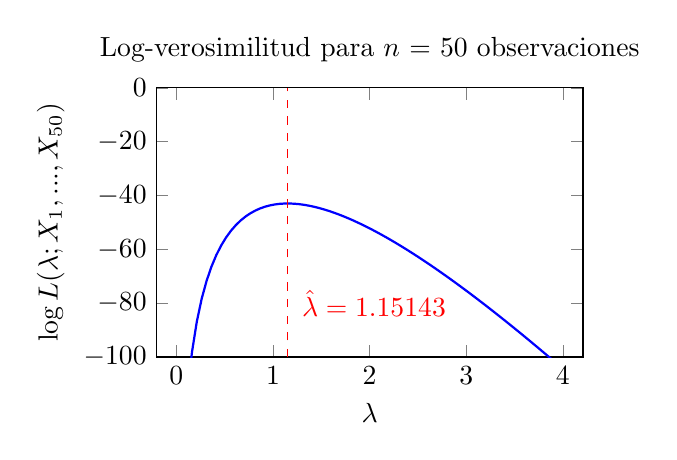
\begin{tikzpicture}
            \begin{axis}[
                domain=0.01:5,
                samples=100,
                ymin=-100, ymax=0,
                xlabel={$\lambda$},
                ylabel={$\log L(\lambda; X_1,...,X_{50})$},
                title={Log-verosimilitud para $n$ = 50 observaciones},
                width=7cm, height=5cm
                ]
                \addplot[thick,blue] {50*ln(x) - x*43.42423};
                \addplot[red, dashed] coordinates {(1.15143, -100) (1.15143, 0)};
                \node at (axis cs: 1.2, -80) [anchor=west, red] {$\hat{\lambda} = 1.15143$};
            \end{axis}
        \end{tikzpicture}

    \end{minipage}

    \begin{center}

        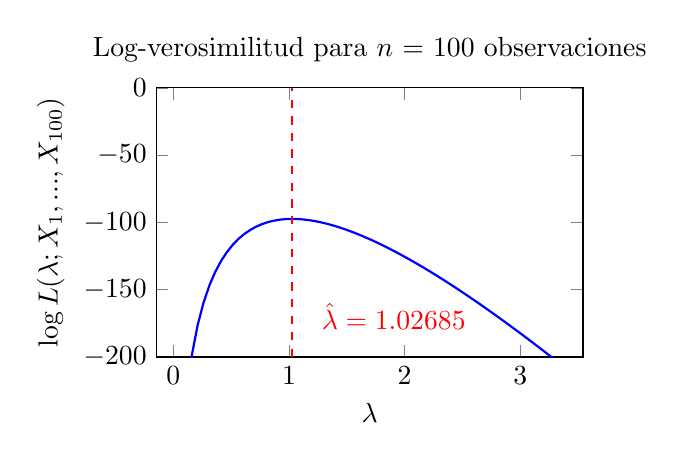
\begin{tikzpicture}
            \begin{axis}[
                domain=0.01:5,
                samples=100,
                ymin=-200, ymax=0,
                xlabel={$\lambda$},
                ylabel={$\log L(\lambda; X_1,...,X_{100})$},
                title={Log-verosimilitud para $n$ = 100 observaciones},
                width=7cm, height=5cm
                ]
                \addplot[thick,blue] {100*ln(x) - x*97.38531};
                \addplot[red, dashed] coordinates {(1.02685, -200) (1.02685, 0)};
                \node at (axis cs: 1.2, -170) [anchor=west, red] {$\hat{\lambda} = 1.02685$};
            \end{axis}
        \end{tikzpicture}
        \caption{Podemos observar como el EMV aproxima el verdadero valor de $\lambda$ en función de la cantidad de observaciones (en este caso $\exp(\lambda)$ donde $\lambda = 1$)}

    \end{center}
    \label{fig:exp-log-ver}
\end{figure}

En la siguiente página se mostrará un ejemplo de como calcular el estimador máximo verosimil de una distribución Bernoulli de parametro $\theta$.

\newpage

\begin{exercise}
    Sean $X_1,\dots,X_n$ v.a.i.i.d. donde $X_i \thicksim B(\theta)$ para $\theta \in (0,1)$. Sea la función de distribución Bernoulli $P_\theta(X=x)=\theta^x(1-\theta)^{1-x}$. Estimar $\theta$ mediante máxima verosimilitud. \\
    Calculamos la verosimilitud como

    \[
        L(\theta;X) \propto \prod_{i=1}^{n}\theta^x(1-\theta)^{1-x}=\theta^{\sum_{i=1}^{n}x_i}(1-\theta)^{n-\sum_{i=1}^{n}x_i}
    \]

    y la log verosimilitud

    \[
        l(\theta; X_1,\dots,X_n)=\sum_{i=1}^{n}x_i\log\theta + (n-\sum_{i=1}^{n}x_i)\log(1-\theta)
    \]

    Encontraremos un máximo en donde se cumpla que $\frac{\partial}{\partial\theta}l(\theta;X_1,\dots,X_n)=0$

    \[
        \frac{\partial}{\partial\theta}l(\theta;X_1,\dots,X_n) = \frac{\sum_{i=1}^{n}x_i}{\theta}-\frac{n-\sum_{i=1}^{n}x_i}{(1-\theta)} \implies
    \]

    \[
        \implies \sum_{i=1}^{n}x_i(1-\theta)=(n-\sum_{i=1}^{n}x_i)\theta \implies \theta=\frac{\sum_{i=1}^{n}x_i}{n}=\overline{X}
    \]

    Por tanto concluimos que el EMV de $\theta$ es $\hat{\theta}=\overline{X}$.

\end{exercise}

\vspace{30pt}

Hilando con la figura \ref{fig:exp-log-ver} donde vemos representada la log verosimilitud de una exponencial, se pondrá como ejemplo también el cálculo del EMV de una distribución exponencial censurada negativa de parámetro $\lambda$.

\textbf{\textit{Definición: }} Sean $X_1, \dots, X_n$ v.a.i.i.d. que siguen una distribución exponencial. Se considera como censura a la derecha cuando se desconoce el tiempo exacto de fallo para $k$ observaciones, pero si se sabe que ocurrió después de un tiempo $t_0$. Es decir, que para $k$ observaciones solo sabemos que $x_i > t_0$.

\vspace{30pt}

Se resolverá el ejercicio en la siguiente página...

\newpage

\begin{exercise}
    Sean $X_1, \dots, X_n$ v.a.i.i.d. donde $X_i$ sigue una exponencial negativa censurada a la derecha de parámetro $\lambda$. Sea la función de distribución exponencial $f(x;\lambda)=\lambda e^{-\lambda x}$. Estimar $\lambda$ mediante máxima verosimilitud. \\
    La función de verosimilitud tendrá dos tipos de datos, los que se obtienen de la exponencial ($f_\lambda(x;\lambda)$) y los $k$ censurados ($P(X_i>t_0)$). \\
    Entonces la función de verosimilitud queda de la siguiente forma:

    \[
        L(\lambda; x_1,\dots,x_n)=\left(\prod_{i=1}^{k}\lambda e^{-\lambda x_i}\right)\left(\prod_{i=k+1}^{n}P(X_i>t_0)\right)
    \]

    Sabemos que

    \[
        P(X_i>t_0)=\int_{t_0}^\infty \lambda e^{-\lambda x}dx = e^{-\lambda t_0}
    \]

    Por lo tanto

    \[
        L(\lambda;x_1,\dots,x_n)=\lambda^k e^{\lambda \sum_{i=1}^{k}x_i}e^{-\lambda(n-k)t_0}
    \]

    Y la log verosimilitud queda

    \[
        l(\lambda;x_1,\dots,x_n)=k\log\lambda-\lambda\left(\sum_{i=1}^{k}x_i + (n-k)t_0\right)
    \]

    Que encontrará máximo en $\hat{\lambda} = \frac{k}{\sum_{i=1}^{k}+(n-k)t_0}$

\end{exercise}

Como último ejemplo se hará lo mismo con la distribución Poisson

\begin{exercise}
    Sean $X_1, \dots, X_n$ v.a.i.i.d. donde $X_i$ sigue una Poisson de parámetro $\lambda$. Sea la función de distribución Poisson $P_\lambda(X=x)=\frac{e^{-\lambda}\lambda^x}{x!}$. Estimar $\lambda$ mediante máxima verosimilitud y comprobar si el estimador es CAN y AE. \\
    La verosimilitud quedará como

    \[
        L(\lambda;x_1,\dots,x_n)=\prod_{i=1}^{n}\frac{e^{-\lambda}\lambda^{x_i}}{{x_i}!}
    \]

    siendo la log verosimilitud

    \[
        l(\lambda; x_1,\dots,x_n)=-n\lambda+\sum_{i=1}^{n}x_i\log\lambda
    \]

    Que encontrará máximo en $\hat{\lambda}=\overline{X}$ \\
    Haciendo uso de este último resultado, es fácil comprobar que $\hat{\lambda}$ es CAN y AE pues

    \[
        \sqrt{n}(\hat{\lambda}-\lambda)=\sqrt{n}(\overline{X}-\lambda) \overset{L}{\to}N(0,\frac{1}{I_1(\lambda)})
    \]

    \[
        I_1(\lambda)=\frac{1}{\lambda} \implies \sqrt{n}(\overline{X}-\lambda)\overset{L}{\to}N(0,\lambda)\square
    \]

\end{exercise}

\newpage

Como generalización del anterior resultado se enuncia el siguiente teorema

\begin{theorem}
    Sean $X_1,\dots,X_n$ v.a.i.i.d. con función de densidad $f(x;\theta)$ donde $\theta \in \Theta$ que verifica CRCR y además que

    \[
        \exists \frac{\partial^3}{\partial \theta^3}\log f(x;\theta) \quad \text{y} \quad \left|\frac{\partial^3}{\partial \theta^3}\log f(x;\theta)\right| \leq M(X); \quad E(M(X))<\infty
    \]

    Entonces el EMV de $\theta$ es CAN y AE. Es decir

    \[
        \sqrt{n}(\hat{\theta}(X)-\theta)\overset{L}{\to}N(0,\frac{1}{I_1(\theta)})
    \]
\end{theorem}

Pongamos un ejemplo

\begin{exercise}
    Sean $X_1, \dots, X_n$ v.a.i.i.d. donde $X_i$ sigue una Normal de parámetros $(0,\sigma^2)$ donde $\sigma^2=\theta$. Sea la función de distribución Normal $f(x;\theta)=\frac{1}{\sqrt(2\pi\theta)}e^{\frac{-x^2}{2\theta}}$. Entonces

    \[
        L(\theta;x_1,\dots,x_n)=\frac{1}{\sqrt{\theta}}e^{\frac{-\sum_{i=1}^{n}x^2_i}{2\theta}} \implies l(\theta;x_1,\dots,x_n)=-\frac{n}{2}\log\theta - \frac{\sum_{i=1}^{n}x^2_i}{2\theta}
    \]

    Que encontrará máximo en $\hat{\theta}=\frac{\sum_{i=1}^{n}x^2_i}{n}$. Entonces

    \[
        \sqrt{n}\left(\frac{\sum_{i=1}^{n}x^2_i}{n}-\theta\right)\overset{L}{\to}N\left(0,\frac{1}{I_1(\theta)}\right)
    \]

    \[
        I_1(\theta)=Var\left(-\frac{n}{2\theta}+\frac{\sum_{i=1}^{n}x^2_i}{2\theta^2}\right)=\frac{n}{2\theta^2}
    \]

    por tanto

    \[
        \sqrt{n}\left(\frac{\sum_{i=1}^{n}x^2_i}{n}-\theta\right) \overset{L}{\to}N(0,2\theta^2) = N(0,2\sigma^4)
    \]
\end{exercise}

Se podría hacer también para una Normal $N(0,\sigma)$ donde $\hat{\theta}=\sqrt{\frac{\sum_{i=1}^{n}x^2_i}{n}}$ que es el EMV para $\sigma$ en modelos $N(0,\sigma)$
Queda como ejercicio para el lector comprobar si

\[
    \sqrt{n}\left(\sqrt{\frac{\sum_{i=1}^{n}x^2_i}{n}}-\sigma\right)\overset{L}{\to}N\left(0,\frac{1}{I_1(\sigma)}\right)
\]
